% ref: https://tikz.net/optics_polarization/
% author: Izaak Neutelings (June 2020)
% Inspiration:
%   https://tex.stackexchange.com/questions/113900/draw-polarized-light
\documentclass[border=3pt,tikz]{standalone}
%\usepackage{amsmath} % for \text
\usepackage{tikz}
\usepackage{physics}
\usepackage{etoolbox} %ifthen
\usetikzlibrary{calc}
\usetikzlibrary{arrows,arrows.meta}
\usetikzlibrary{angles,quotes} % for pic (angle labels)
%\input{arrowsnew}
%\renewcommand{\familydefault}{\sfdefault}
\tikzset{>=latex} % for LaTeX arrow head

\newcommand\degree{^\circ}
\colorlet{crystal}{blue!75}
\colorlet{vcol}{green!50!black}
\colorlet{Ecol}{orange!90!black}
\colorlet{EWcol}{orange!80!black}
\colorlet{EVcol}{orange!80!black!60}
\def\zangle{-20}
\def\xangle{20}
\tikzstyle{platecol}=[blue!80!black!40,opacity=0.8]
\tikzstyle{platetopcol}=[blue!90!black!50,opacity=0.8]
\tikzstyle{platesidEcol}=[blue!70!black!50,opacity=0.8]
\tikzstyle{mydashed}=[dash pattern=on 1.2 off 0.7,line width=0.3]
\tikzstyle{Evec}=[EVcol,-{Stealth[length=1.8,width=1.2]},line width=0.2]
%\tikzstyle{Evec}=[EVcol,-stealth,line width=0.2]
%\tikzstyle{Evec}=[EVcol,-{>[scale=0.2]},line width=0.2]
%\tikzstyle{Evec}=[EVcol,-latexnew,arrowhead=1,line width=0.2]

% RIGHT ANGLE
\newcommand\rightAngle[4]{
  \pgfmathanglebetweenpoints{\pgfpointanchor{#2}{center}}{\pgfpointanchor{#3}{center}}
  \coordinate (tmpRA) at ($(#2)+(\pgfmathresult+45:#4)$);
  \draw[white,line width=0.6] ($(#2)!(tmpRA)!(#1)$) -- (tmpRA) -- ($(#2)!(tmpRA)!(#3)$);
  \draw[blue!40!black] ($(#2)!(tmpRA)!(#1)$) -- (tmpRA) -- ($(#2)!(tmpRA)!(#3)$);
}

% POLARIZER
\def\W{3.5}  % width polarizer
\def\w{0.05} % width slit
\def\l{2.9}  % length slit
\def\t{0.05}
\def\N{7}    % number of slits
\tikzset{
  plate/.pic={
%    \fill[platetopcol]
%      (-\W/2,\W/2,0) --++ (\W,0,0) --++ (0,0,-\t) --++ (-\W,0,0) -- cycle;
%    \fill[platesidEcol]
%      (-\W/2,-\W/2,0) --++ (0,\W,0) --++ (0,0,-\t) --++ (0,-\W,0) -- cycle;
%    \fill[platecol,even odd rule]
%      (-\W/2,-\W/2,0) --++ (\W,0,0) --++ (0,\W,0) --++ (-\W,0,0) -- cycle
%      \foreach \i [evaluate={\x=-\W/2+\i*\W/(\N+1);}] in {1,...,\N}{
%        (\x-\w/2,-\l/2) --++ (0,\l) --++ (\w,0) --++ (0,-\l) -- cycle
%      };
    \ifnumless{45}{#1}{
      \def\topang{#1}
    }{
      \def\topang{#1+90}
    }
    \fill[platetopcol]
      (\topang:\W/2)++(\topang-90:\W/2) --++ (0,0,-\t) --++ (\topang+90:\W) --++ (0,0,\t) -- cycle;
    \fill[platesidEcol]
      (\topang+90:\W/2)++(\topang:\W/2) --++ (0,0,-\t) --++ (\topang+180:\W) --++ (0,0,\t) -- cycle;
    \fill[platecol]
      (#1:\W/2)++(#1-90:\W/2) --++ (#1-180:\W) --++ (#1+90:\W) --++ (#1:\W) -- cycle
      \foreach \i [evaluate={\x=-\W/2+\i*\W/(\N+1);}] in {1,...,\N}{
        (#1:\l/2)++(#1+90:\x+\w/2) --++ (#1-180:\l) --++ (#1-90:\w) --++ (#1:\l) -- cycle
      };
  }
}


\begin{document}


% POLARIZATION: 90, theta
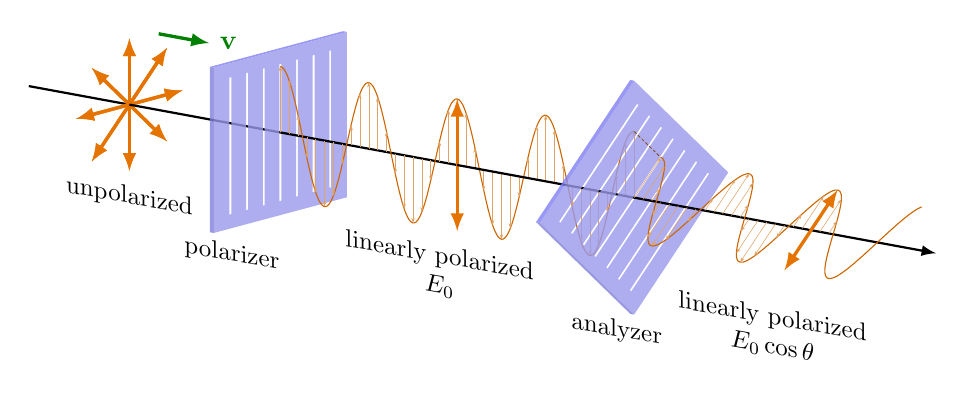
\begin{tikzpicture}[x=(15:0.5), y=(90:0.6), z=(-20:2.2)]
  
  \def\A{1.4}
  \def\L{3.2}
  \def\M{4.5}
  \def\nwave{4}
  \def\k{(360*\nwave/\M)} % 2pi*n / L = 360*n / L
  %\def\dx{90/\k}
  \def\nvec{40} % per wavelength
  
  % SECTION 1
  \draw[thick] (0,0,0) -- (0,0,0.4*\L);
  \foreach \ang in {45,90,...,360}{
    \draw[<->,very thick,Ecol] (0,0,0.4*\L)++(\ang:\A) --++ (\ang+180:2*\A);
  }
  %\node[Ecol,above] at (45:\A) {$\vb{E}$};
  \draw[thick] (0,0,0.4*\L) -- (0,0,\L);
  \draw[->,very thick,vcol] (0,0,0.4*\L)++(60:1.1*\A) --++ (0,0,0.2*\L) node[right] {$\vb{v}$};
  \node[scale=0.9,yslant=tan(-10)] at (0,-1.4*\A,0.4*\L) {unpolarized};
  
  % SECTION 2
  \begin{scope}[shift={(0,0,\L)}]
    \pic at (0,0) {plate={90}};
    \node[scale=0.9,yslant=tan(-10),right=7,below] at (-135:0.7*\W) {polarizer};
    \draw[thick] (0,0,0) -- (0,0,\M/2);
    \draw[<->,very thick,Ecol] (0,0,\M/2)++(90:\A) --++ (-90:2*\A); %-\dx
    \draw[EWcol,samples=100,smooth,variable=\z,domain=0:\M]
      plot(0,{\A*cos(\k*\z)},\z);
    \foreach \i [evaluate={\z=\i*\M/\nvec; \c=int(\i!=\nvec/2);}] in {0,...,\nvec}{
      \ifnum\c=1
        \draw[Evec] (0,0,\z) --++ (90:{\A*cos(\k*\z)});
      \fi
    }
    \draw[thick] (0,0,\M/2) -- (0,0,\M);
    \node[scale=0.9,yslant=tan(-10),below=-7,align=center] at (0,-1.4*\A,0.45*\M)
      {linearly polarized\\$E_0$};
  \end{scope}
  
  % SECTION 3
  \begin{scope}[shift={(0,0,\L+\M)}]
    \pic at (0,0) {plate={45}};
    \node[scale=0.9,yslant=tan(-10),left=7,below] at (-90:0.7*\W) {analyzer};
    \draw[->,thick] (0,0,0) -- (0,0,1.2*\L);
    \draw[<->,very thick,Ecol] (0,0,\M/2)++(45:{\A*cos(45)}) --++ (-135:{2*\A*cos(45)}); %-\dx
    \draw[Ecol!50!black!90,mydashed]
      (90:\A) -- (45:{\A*cos(45)});
    \draw[EWcol,samples=100,smooth,variable=\z,domain=0:0.74*\M]
      plot({\A*cos(\k*\z)*cos(45)^2},{\A*cos(\k*\z)*cos(45)^2},\z);
    \foreach \i [evaluate={\z=\i*\M/\nvec; \c=int(\i!=\nvec/2 && \i<23);}] in {0,...,\nvec}{
      \ifnum\c=1
        \draw[Evec] (0,0,\z) --++ (45:{\A*cos(\k*\z)*cos(45)});
      \fi
    }
    \node[scale=0.9,yslant=tan(-10),below=-7,align=center] at (0,-1.4*\A,0.55*\L)
      {linearly polarized\\$E_0\cos\theta$};
  \end{scope}
  
\end{tikzpicture}



% POLARIZATION: 90, 0
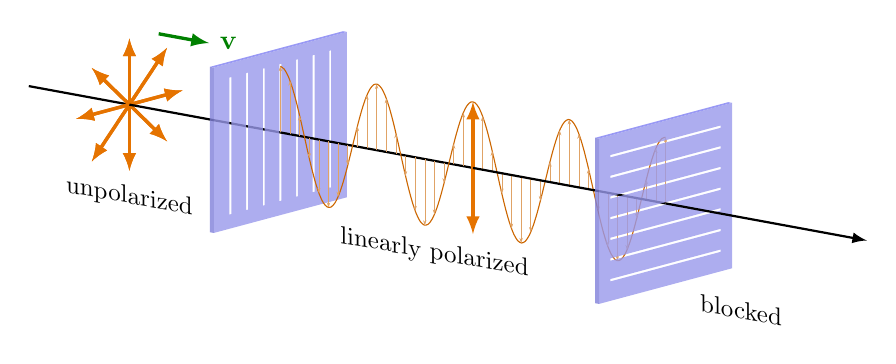
\begin{tikzpicture}[x=(15:0.5), y=(90:0.6), z=(-20:2.2)]
  
  \def\A{1.4}
  \def\L{3.2}
  \def\M{4.9}
  \def\nwave{4}
  \def\k{(360*\nwave/\M)} % 2pi*n / L = 360*n / L
  %\def\dx{90/\k}
  \def\nvec{40} % per wavelength
  
  % SECTION 1
  \draw[thick] (0,0,0) -- (0,0,0.4*\L);
  \foreach \ang in {45,90,...,360}{
    \draw[<->,very thick,Ecol] (0,0,0.4*\L)++(\ang:\A) --++ (\ang+180:2*\A);
  }
  %\node[Ecol,above] at (45:\A) {$\vb{E}$};
  \draw[thick] (0,0,0.4*\L) -- (0,0,\L);
  \draw[->,very thick,vcol] (0,0,0.4*\L)++(60:1.1*\A) --++ (0,0,0.2*\L) node[right] {$\vb{v}$};
  \node[scale=0.9,yslant=tan(-10)] at (0,-1.4*\A,0.4*\L) {unpolarized};
  
  % SECTION 2
  \begin{scope}[shift={(0,0,\L)}]
    \pic at (0,0) {plate={90}};
    \draw[thick] (0,0,0) -- (0,0,\M/2);
    \draw[<->,very thick,Ecol] (0,0,\M/2)++(90:\A) --++ (-90:2*\A); %-\dx
    \draw[EWcol,samples=100,smooth,variable=\z,domain=0:\M]
      plot(0,{\A*cos(\k*\z)},\z);
    \foreach \i [evaluate={\z=\i*\M/\nvec; \c=int(\i!=\nvec/2);}] in {0,...,\nvec}{
      \ifnum\c=1
        \draw[Evec] (0,0,\z) --++ (90:{\A*cos(\k*\z)});
      \fi
    }
    \draw[thick] (0,0,\M/2) -- (0,0,\M);
    \node[scale=0.9,yslant=tan(-10)] at (0,-1.4*\A,0.4*\M) {linearly polarized};
  \end{scope}
  
  % SECTION 3
  \begin{scope}[shift={(0,0,\L+\M)}]
    \pic at (0,0) {plate={0}};
    \draw[->,thick] (0,0,0) -- (0,0,0.8*\L);
    \node[scale=0.9,yslant=tan(-10)] at (0,-1.4*\A,0.3*\L) {blocked};
  \end{scope}
  
\end{tikzpicture}



% POLARIZATION: 90, 45, 0
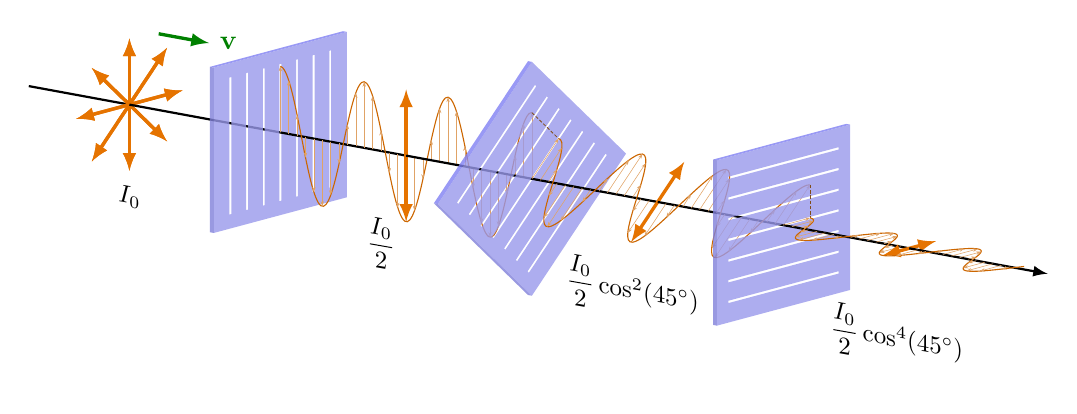
\begin{tikzpicture}[x=(15:0.5), y=(90:0.6), z=(-20:2.2)]
  
  \def\A{1.4}
  \def\L{3.2}
  \def\nwave{3}
  \def\k{(360*\nwave/\L)} % 2pi*n / L = 360*n / L
  %\def\dx{90/\k}
  \def\nvec{30} % per wavelength
  
  % SECTION 1
  \draw[thick] (0,0,0) -- (0,0,0.4*\L);
  \foreach \ang in {45,90,...,360}{
    \draw[<->,very thick,Ecol] (0,0,0.4*\L)++(\ang:\A) --++ (\ang+180:2*\A);
  }
  %\node[Ecol,above] at (45:\A) {$\vb{E}$};
  \draw[thick] (0,0,0.4*\L) -- (0,0,\L);
  \draw[->,very thick,vcol] (0,0,0.4*\L)++(60:1.1*\A) --++ (0,0,0.2*\L) node[right] {$\vb{v}$};
  \node[scale=0.9,yslant=tan(-10)] at (0,-1.4*\A,0.4*\L) {$I_0$}; %,align=center
  
  % SECTION 2
  \begin{scope}[shift={(0,0,\L)}]
    \pic at (0,0) {plate={90}};
    \draw[thick] (0,0,0) -- (0,0,\L/2);
    \draw[<->,very thick,Ecol] (0,0,\L/2)++(90:\A) --++ (-90:2*\A); %-\dx
    \draw[EWcol,samples=100,smooth,variable=\z,domain=0:\L]
      plot(0,{\A*cos(\k*\z)},\z);
    \foreach \i [evaluate={\z=\i*\L/\nvec; \c=int(\i!=\nvec/2);}] in {0,...,\nvec}{
      \ifnum\c=1
        \draw[Evec] (0,0,\z) --++ (90:{\A*cos(\k*\z)});
      \fi
    }
    \draw[thick] (0,0,\L/2) -- (0,0,\L);
    \node[scale=0.9,yslant=tan(-10)] at (0,-1.4*\A,0.4*\L) {$\dfrac{I_0}{2}$}; %, $90\degree$
  \end{scope}
  
  % SECTION 3
  \begin{scope}[shift={(0,0,2*\L)}]
    \pic at (0,0) {plate={45}};
    \draw[thick] (0,0,0) -- (0,0,\L/2);
    \draw[<->,very thick,Ecol] (0,0,\L/2)++(45:{\A*cos(45)}) --++ (225:{2*\A*cos(45)}); %-\dx
    \draw[thick] (0,0,\L/2) -- (0,0,\L);
    \draw[Ecol!50!black!90,mydashed]
      (90:\A) -- (45:{\A*cos(45)});
    \draw[EWcol,samples=100,smooth,variable=\z,domain=0:\L]
      plot({\A*cos(\k*\z)*cos(45)^2},{\A*cos(\k*\z)*cos(45)^2},\z);
    \foreach \i [evaluate={\z=\i*\L/\nvec; \c=int(\i!=\nvec/2);}] in {0,...,\nvec}{
      \ifnum\c=1
        \draw[Evec] (0,0,\z) --++ (45:{\A*cos(\k*\z)*cos(45)});
      \fi
    }
    \node[scale=0.9,yslant=tan(-10)] at (0,-1.4*\A,0.4*\L) {$\dfrac{I_0}{2}\cos^2(45\degree)$}; %, $45\degree$
  \end{scope}
  
  % SECTION 4
  \begin{scope}[shift={(0,0,3*\L)}]
    \pic at (0,0) {plate={0}};
    \draw[thick] (0,0,0) -- (0,0,\L/2);
    \draw[Evec] (0,0,14*\L/\nvec) --++ (0:{\A*cos(\k*14*\L/\nvec)*cos(45)^2}); % put behind big arrow
    \draw[<->,very thick,Ecol] (0,0,\L/2)++(0:{\A*cos(45)^2}) --++ (180:{2*\A*cos(45)^2}); %-\dx
    \draw[->,thick] (0,0,\L/2) -- (0,0,1.05*\L);
    \draw[Ecol!50!black!90,mydashed]
      (45:{\A*cos(45)}) -- (0:{\A*cos(45)^2});
    \draw[EWcol,samples=100,smooth,variable=\z,domain=0:0.93*\L]
      plot({\A*cos(\k*\z)*cos(45)^2},0,\z);
    \foreach \i [evaluate={
        \z=\i*\L/\nvec;
        \c=int(\i!=\nvec/2 && \i!=\nvec/2-1 && \i<\nvec-2);
      }] in {0,...,\nvec}{
      \ifnum\c=1
        \draw[Evec] (0,0,\z) --++ (0:{\A*cos(\k*\z)*cos(45)^2});
      \fi
    }
    \node[scale=0.9,yslant=tan(-10)] at (0,-1.4*\A,0.45*\L) {$\dfrac{I_0}{2}\cos^4(45\degree)$}; %, $0\degree$
  \end{scope}
  
\end{tikzpicture}



% POLARIZER projection
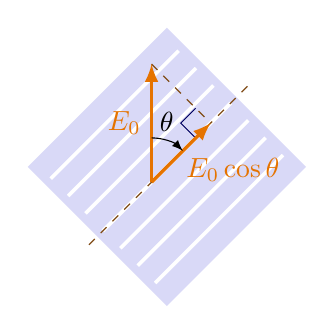
\begin{tikzpicture}
  \def\W{2.5}  % width polarizer
  \def\w{0.05} % width slit
  \def\l{2.3}  % length slit
  \def\N{7}    % number of slits
  \def\A{1.5}  % amplitude/size E vector
  \def\ang{45} % angle polarizer
  \coordinate (O) at (0,0);
  \coordinate (E0) at (90:\A);
  \coordinate (E) at (45:{\A*cos(45)});
  
  \fill[blue!80!black!15,shift={(45:0.11*\W)}]
    (\ang:\W/2)++(\ang-90:\W/2) --++ (\ang-180:\W) --++ (\ang+90:\W) --++ (\ang:\W) -- cycle
    \foreach \i [evaluate={\x=-\W/2+\i*\W/(\N+1);}] in {1,...,\N}{
      (\ang:\l/2)++(\ang+90:\x+\w/2) --++ (\ang-180:\l) --++ (\ang-90:\w) --++ (\ang:\l) -- cycle
    };
  
  \draw[Ecol!50!black!90,dashed] (-135:0.75*\A) -- (45:1.2*\A) coordinate (T);
  \draw[Ecol!50!black!90,dashed] (90:\A) -- (45:{\A*cos(45)});
  \rightAngle{O}{E}{E0}{0.38}
  \draw[->,Ecol,very thick] (0,0) -- (E0) node[midway,left] {$E_0$};
  \draw[->,Ecol,very thick] (0,0) -- (E) node[midway,below right=-2] {$E_0 \cos\theta$}; %45\degree
  \draw pic[<-,"$\theta$"{anchor=-85},draw=black,angle radius=16,angle eccentricity=1] {angle = E--O--E0};
  
\end{tikzpicture}



%% EXAMPLE
%% Source: https://tex.stackexchange.com/questions/113900/draw-polarized-light
%\begin{tikzpicture}[x=(\xangle:0.75cm), y=(90:1cm), z=(\zangle:1.5cm),
%    >=stealth, line cap=round, line join=round,
%    lines/.style={gray!50, thick}, 
%    axis/.style={black, thick},
%    plate/.style={fill, opacity=0.875},
%    markers/.style={orange, thick}]
%
%  \node [yslant=tan(\zangle), above=0.25cm, align=center,font=\small] at 
%    (1,1,1.5){Left Handed \\ Circularly Polarized Light};
%
%  \draw [lines] (-1,-1,0) -- (-1,1,0) -- (1,1,0) -- (1,-1, 0) -- cycle;
%  \draw [lines] (1,0,0) \foreach \t in {0,5,...,355}{
%        -- (cos \t, sin \t, 0) } -- cycle;
%  
%  \draw [lines] (1,1,0) -- (1,1,3.125);
%  \draw [lines] (-1,-1,0) -- (-1,-1,3.125);
%  \draw [axis, ->] (0,0,3.125) -- (0,0,0);
%  
%  \foreach \k [evaluate={%
%    \i=\k*5.625; 
%    \j=\i>0 ? \i-5.625 : 0; 
%    \a=90-\i; 
%    \b=90-\j; 
%    \c=int(mod(\k,4));}] 
%    in {0,...,192}{
%        \ifnum\c=0
%            \draw [->] (0,0,\i/360) -- ++(cos \a, sin \a, 0);
%        \fi
%        \draw [red] (cos \a, sin \a, \i/360) -- (cos \b, sin \b, \j/360);
%    }
%  
%  \begin{scope}[shift={(0,0,3.125)}]
%  
%    \node [yslant=tan(\zangle), above=0.25cm, align=center,font=\small] at 
%      (1,1,1.5){Linearly Polarized Light};
%  
%    \begin{scope}[xscale=1.5, yscale=1.5]
%      \path [crystal!25, plate] 
%        (-1,-1,0) -- (-1,1,0) -- (1,1,0) -- (1,-1,0) -- cycle;
%      \path [crystal!50, plate] 
%        (-1,-1,0) -- (-1,-1,-0.125) -- (-1,1,-0.125) -- (-1,1, 0) -- cycle;
%      \path [crystal!75, plate] 
%        (-1,1,0) -- (-1,1,-0.125) -- (1,1,-0.125) -- (1,1, 0) -- cycle;
%      \node [yslant=tan(\xangle), text=crystal!50, below, font=\small] at 
%        (-1.125,-1,0){Quarter Wave Plate};
%    \end{scope}
%    
%    \draw [markers] (0,1) -- (0,-1) (-0.5,0) -- (0.5,0);
%    \draw [lines] (1,1,0) -- (1,1,3);
%    \draw [lines] (-1,-1,0) -- (-1,-1,3);
%    
%    \draw [axis] (0,0,0) -- (0,0,3);
%    
%    \foreach \k [evaluate={%
%      \i=\k*5.625; \j=\i>0 ? \i-5.625 : 0; 
%      \a=90-\i; 
%      \b=90-\j; 
%      \c=int(mod(\k,4)==0 && sin \a != 0); 
%      \d=int(\k+1/4);}] in {0,...,192}{
%      \ifodd\d
%        \ifnum\c=1
%          \draw [->] (0,0,\i/360) -- ++(sin \a, sin \a, 0);
%        \fi
%        \draw [red] (sin \a, sin \a, \i/360) -- (sin \b, sin \b, \j/360);
%      \else
%        \draw [red] (sin \a, sin \a, \i/360) -- (sin \b, sin \b, \j/360);
%        \ifnum\c=1
%          \draw [->] (0,0,\i/360) -- ++(sin \a, sin \a, 0);
%        \fi
%      \fi
%    }
%  \end{scope}
%  
%  \begin{scope}[shift={(0,0,6.125)}]
%    
%    \node [yslant=tan(\zangle), above=0.25cm, align=center,font=\small]
%      at (1,1,1.5){Unpolarized Light};
%    
%    \begin{scope}[xscale=1.5, yscale=1.5]
%      \path [crystal!25, plate] 
%        (-1,-1,0) -- (-1,1,0) -- (1,1,0) -- (1,-1, 0) -- cycle;
%      \path [crystal!50, plate] 
%        (-1,-1,0) -- (-1,-1,-0.0625) -- (-1,1,-0.0625) -- (-1,1, 0) -- 
%        cycle;
%      \path [crystal!75, plate] 
%        (-1,1,0) -- (-1,1,-0.0625) -- (1,1,-0.0625) -- (1,1, 0) -- cycle;
%      \node [yslant=tan(\xangle), text=crystal!50, below, font=\small] at 
%        (-1,-1,0){Linear Polarizer};
%    \end{scope}
%    
%    \draw [markers] (-1.25,-1.25) -- (1.25,1.25);
%    \draw [lines] (0,1.414,0) -- (0,1.414,2);
%    \draw [lines] (1.414,0,0) -- (1.414,0,3);
%    \draw [lines] (1,1,0) -- (1,1,1);
%    \draw [lines] (-1,-1,0) -- (-1,-1, 0.5);
%    \draw [axis] (0,0,0) -- (0,0,3);
%    
%    \foreach \k [evaluate={%
%      \i=\k*5.625; \j=\i>0 ? \i-5.625 : 0;
%      \a=90-\i; 
%      \b=90-\j; 
%      \c=int((mod(\k,4)==0 && sin \a != 0) || (\k==65) || (\k==129)); 
%      \d=int(\k+1/4);
%      \r=(\k>64) ? 1.414 : 1;
%      \xa=(\k > 64) && (\k < 129) ? 0 : sin(\a)*\r;
%      \xb=(\k > 64) && (\k < 129) ? 0 : sin(\b)*\r;
%      \ya=(\k < 129) ? sin(\a)*\r : 0;
%      \yb=(\k < 129) ? sin(\b)*\r : 0;
%      }] in {0,...,192}{
%      \ifodd\d
%        \ifnum\c=1
%          \draw [->] (0,0,\i/360) -- ++(\xa, \ya, 0);
%        \fi
%        \draw [red] (\xa, \ya, \i/360) -- (\xb, \yb, \j/360);
%      \else
%        \draw [red] (\xa, \ya, \i/360) -- (\xb, \yb, \j/360);
%        \ifnum\c=1
%          \draw [->] (0,0,\i/360) -- ++(\xa, \ya, 0);
%        \fi
%      \fi
%    }
%    
%    \draw [ultra thick, ->] (0,0,3.5) -- (0,0,3);
%  
%  \end{scope}
%  
%\end{tikzpicture}



\end{document}